\section{Virtual Layer Design}
In this section, we introduce specific managements in the virtual layer for unified virtual RDMA.

\subsection{vRNIC Mapping Management}
The same virtual layer needs to create multiple vRNICs and provide them to different containers or virtual machines respectively. If each vRNIC is directly mapped to the same RNIC, it will compete for the same PCIe bus and share the configuration space of RNIC. The vRNICs are still not isolated or limited.

SR-IOV is a popular hardware-based virtualization technology. RNIC can virtualize multiple different hardware interface, called VFs. Each VF has a unique PCIe bus and configuration space. At the same time, when configuring VFs, users can limit network rate and other hardware resources, and implement management policies such as QoS. The uniRDMA virtual layer maps each vRNIC to the VF interface of RNIC separately, so hardware-level isolation is guaranteed for vRNICs.

However, the VF resources of SR-IOV are limited, for example, only 126 VFs are supported in Mellanox ConnectX-3 at most~\cite{ofed-manual}. Therefore, the existing VFs need to be managed and coordinated in a unified to meet many vRNICs.

\begin{figure}[!ht]
	\centering
	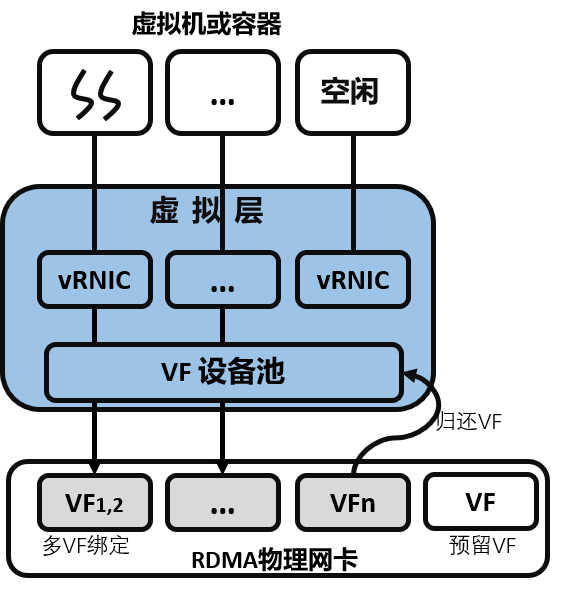
\includegraphics[width=0.9\linewidth]{images/vf-mapping}
	\caption{Management of vRNIC Mapping}
	\label{fig:vf-mapping}
\end{figure}

As Figure~\ref{fig:vf-mapping} shows: First, the virtual layer constructs a dynamic VF pool. The initial number of VFs in the pool is usually the number of pre-determined virtual instances. If lack of free VFs in the pool, the device pool can dynamically expand the number of VFs. Second, the virtual layer supports dynamic mapping between vRNIC and VF. When all virtual RDMA resources have been destroyed, the virtual layer marks the VF as idle and puts it back into the pool. So that the virtual layer can support the number of vRNICs that exceed the VF limit. Finally, the virtual layer supports various mapping relationships between vRNICs and VFs. For example, load balancing can be meted by map a vRNIC with multiple VFs. VF resources are saved by mapping multiple vRNICs of the same virtual instance to the single VF. 


\subsection{Virtual RDMA Management}
To maintain portability and realize RDMA network management, RDMA connections between vRNICs cannot be established by the physical address of VFs. But this problem has a solution that uniRDMA virtual layer acts as a software RDMA switch or router for virtual RDMA network configuration and routing management, etc.

RNICs are usually managed by the subnet manager in the cluster. For the same purpose, a control center is set up in uniRDMA to assign virtual RDMA addresses vGIDs to each vRNIC and configure routing rules between vRNICs. As shown in Figure~\ref{fig:route-config} , the vRNICs are divided into two groups: group 1 and group 2; vRNICs in the same group are allowed to establish RDMA connections, and cross-group RDMA connections cannot succeed due to the isolated routing rules between group 1 and group 2.

\begin{figure}[!ht]
	\centering
	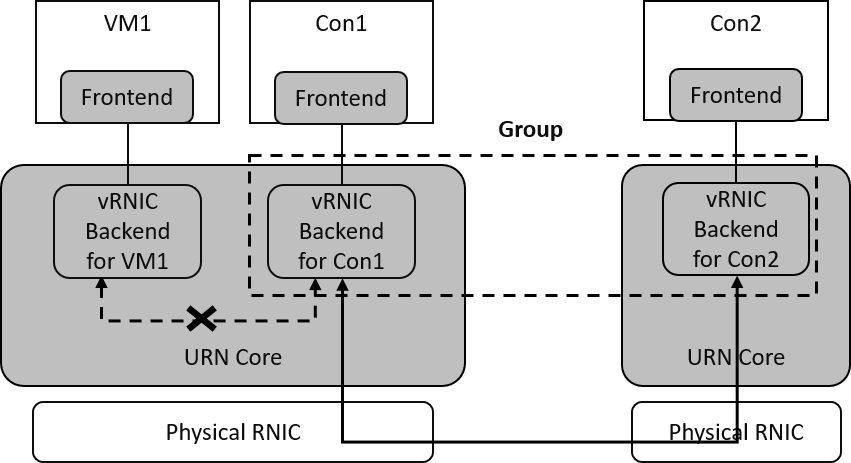
\includegraphics[width=1.0\linewidth]{images/route-config}
	\caption{Virtual RDMA Network Routing}
	\label{fig:route-config}
\end{figure}

Consistent with native RDMA, vRNICs in each virtual layer need to exchange each other's virtual RDMA addresses, virtual QP queue information, registered memory keys and other information to establish virtual RDMA connections. However, the vRNIC RDMA address is virtual, and does not recognized in RNIC. Therefore, the mapping relations between the virtual addresses of vRNICs and the physical addresses of VF needs to be exchanged between virtual layers. When establishing the virtual RDMA connection, the virtual RDMA address is converted to the physical address of the mapped VFs. Note that RDMA resources information, such as virtual QP number and memory keys, have been mapped to the VF interface by the map unit in vRNIC, they can all be recognized VF and directly used to create RDMA connection.
